% Options for packages loaded elsewhere
% Options for packages loaded elsewhere
\PassOptionsToPackage{unicode}{hyperref}
\PassOptionsToPackage{hyphens}{url}
\PassOptionsToPackage{dvipsnames,svgnames,x11names}{xcolor}
%
\documentclass[
  11pt,
]{article}
\usepackage{xcolor}
\usepackage[top=0.4in,bottom=0.45in,left=0.65in,right=0.65in,includehead,headheight=52pt,headsep=7pt,includefoot,footskip=24pt]{geometry}
\usepackage{amsmath,amssymb}
\setcounter{secnumdepth}{-\maxdimen} % remove section numbering
\usepackage{iftex}
\ifPDFTeX
  \usepackage[T1]{fontenc}
  \usepackage[utf8]{inputenc}
  \usepackage{textcomp} % provide euro and other symbols
\else % if luatex or xetex
  \usepackage{unicode-math} % this also loads fontspec
  \defaultfontfeatures{Scale=MatchLowercase}
  \defaultfontfeatures[\rmfamily]{Ligatures=TeX,Scale=1}
\fi
\usepackage{lmodern}
\ifPDFTeX\else
  % xetex/luatex font selection
\fi
% Use upquote if available, for straight quotes in verbatim environments
\IfFileExists{upquote.sty}{\usepackage{upquote}}{}
\IfFileExists{microtype.sty}{% use microtype if available
  \usepackage[]{microtype}
  \UseMicrotypeSet[protrusion]{basicmath} % disable protrusion for tt fonts
}{}
\makeatletter
\@ifundefined{KOMAClassName}{% if non-KOMA class
  \IfFileExists{parskip.sty}{%
    \usepackage{parskip}
  }{% else
    \setlength{\parindent}{0pt}
    \setlength{\parskip}{6pt plus 2pt minus 1pt}}
}{% if KOMA class
  \KOMAoptions{parskip=half}}
\makeatother
% Make \paragraph and \subparagraph free-standing
\makeatletter
\ifx\paragraph\undefined\else
  \let\oldparagraph\paragraph
  \renewcommand{\paragraph}{
    \@ifstar
      \xxxParagraphStar
      \xxxParagraphNoStar
  }
  \newcommand{\xxxParagraphStar}[1]{\oldparagraph*{#1}\mbox{}}
  \newcommand{\xxxParagraphNoStar}[1]{\oldparagraph{#1}\mbox{}}
\fi
\ifx\subparagraph\undefined\else
  \let\oldsubparagraph\subparagraph
  \renewcommand{\subparagraph}{
    \@ifstar
      \xxxSubParagraphStar
      \xxxSubParagraphNoStar
  }
  \newcommand{\xxxSubParagraphStar}[1]{\oldsubparagraph*{#1}\mbox{}}
  \newcommand{\xxxSubParagraphNoStar}[1]{\oldsubparagraph{#1}\mbox{}}
\fi
\makeatother


\usepackage{longtable,booktabs,array}
\newcounter{none} % for unnumbered tables
\usepackage{calc} % for calculating minipage widths
% Correct order of tables after \paragraph or \subparagraph
\usepackage{etoolbox}
\makeatletter
\patchcmd\longtable{\par}{\if@noskipsec\mbox{}\fi\par}{}{}
\makeatother
% Allow footnotes in longtable head/foot
\IfFileExists{footnotehyper.sty}{\usepackage{footnotehyper}}{\usepackage{footnote}}
\makesavenoteenv{longtable}
\usepackage{graphicx}
\makeatletter
\newsavebox\pandoc@box
\newcommand*\pandocbounded[1]{% scales image to fit in text height/width
  \sbox\pandoc@box{#1}%
  \Gscale@div\@tempa{\textheight}{\dimexpr\ht\pandoc@box+\dp\pandoc@box\relax}%
  \Gscale@div\@tempb{\linewidth}{\wd\pandoc@box}%
  \ifdim\@tempb\p@<\@tempa\p@\let\@tempa\@tempb\fi% select the smaller of both
  \ifdim\@tempa\p@<\p@\scalebox{\@tempa}{\usebox\pandoc@box}%
  \else\usebox{\pandoc@box}%
  \fi%
}
% Set default figure placement to htbp
\def\fps@figure{htbp}
\makeatother





\setlength{\emergencystretch}{3em} % prevent overfull lines

\providecommand{\tightlist}{%
  \setlength{\itemsep}{0pt}\setlength{\parskip}{0pt}}



 


% =====================================================================
%  _style.tex  ·  Design system for EIL research highlights (v8 layout)
%  Edit here to restyle ALL research highlights. Included via the .qmd YAML.
%  Matches the canonical single-column v8 template; the masthead and footer
%  are set per-document via fancyhdr in each .qmd's include-in-header.
% =====================================================================

% ---- Colours (exact hex) --------------------------------------------
\definecolor{ink}{HTML}{1D2620}        % title, masthead rule
\definecolor{body}{HTML}{33352C}       % main body paragraphs
\definecolor{accentred}{HTML}{641111}  % RESEARCH HIGHLIGHT label, links, section heads, fig title
\definecolor{boxred}{HTML}{8C2826}     % Bottom Line box fill
\definecolor{boxtext}{HTML}{EEF1EA}    % Bottom Line body text (off-white)
\definecolor{muted}{HTML}{50534A}      % figure source line
\definecolor{cite}{HTML}{6E6D61}       % citation line
\definecolor{faint}{HTML}{9A978A}      % footer
\definecolor{warmrule}{HTML}{D8D2C2}   % thin warm-grey dividers
\definecolor{paper}{HTML}{FAF8F1}      % warm page background

% \pagecolor{paper}                    % uncomment for warm off-white background

% ---- Fonts (Source Sans 3 / Source Serif 4) -------------------------
\usepackage[T1]{fontenc}
\usepackage[default]{sourcesanspro}
\usepackage{sourceserifpro}
\renewcommand{\familydefault}{\sfdefault}

% ---- Page -----------------------------------------------------------
\pagestyle{empty}
\setlength{\parindent}{0pt}
\setlength{\parskip}{2pt}
% Default body size/colour. The .qmd overrides this to 10.5/13.5pt.
\AtBeginDocument{\color{body}\fontsize{9.4pt}{13.6pt}\selectfont}

% ---- Packages -------------------------------------------------------
\usepackage{microtype}
\usepackage{soul}
\setul{2pt}{.5pt}
\usepackage{tcolorbox}
\tcbuselibrary{skins}
\usepackage[colorlinks=true, urlcolor=accentred, linkcolor=accentred, pdfborder={0 0 0}]{hyperref}

% =====================================================================
%  MACROS
% =====================================================================

% --- Title + citation (citation has a thin warm divider beneath) ------
\newcommand{\brieftitle}[1]{%
  {\color{ink}\fontsize{18pt}{19.5pt}\selectfont\bfseries\textls[-12]{#1}\par}\vspace{3pt}}
\newcommand{\briefcitation}[1]{%
  {\color{cite}\fontsize{9.4pt}{12pt}\selectfont #1\par}\vspace{3pt}%
  \noindent\textcolor{warmrule}{\rule{\linewidth}{0.7pt}}}

% --- Section heads (uppercase, maroon) -------------------------------
\newcommand{\sectionhead}[1]{%
  \vspace{2pt}{\color{accentred}\bfseries\fontsize{9.75pt}{12pt}\selectfont
  \textls[20]{\MakeUppercase{#1}}\par}\vspace{1pt}}

% --- Sub-heads (small uppercase) -------------------------------------
% Legacy — the retired Takeaways block used these. Kept in the brand
% maroon so older highlights that call \subhead still compile.
\newcommand{\subhead}[1]{%
  {\color{accentred}\bfseries\fontsize{8.25pt}{10pt}\selectfont
  \textls[50]{\MakeUppercase{#1}}\par}\vspace{2pt}}

% --- Figure title + source line --------------------------------------
\newcommand{\figtitle}[2]{%
  {\bfseries\color{accentred}\fontsize{7.1pt}{9pt}\selectfont\textls[40]{\MakeUppercase{#1}}}\par%
  {\color{muted}\fontsize{7.1pt}{9pt}\selectfont #2}\par\vspace{4pt}}

% =====================================================================
%  COLOURED BOXES
% =====================================================================

% --- Bottom Line box (border-radius 6px -> arc=4pt) ------------------
\newtcolorbox{bottomline}{%
  enhanced, arc=4pt, outer arc=4pt, boxrule=0pt,
  colback=boxred, coltext=boxtext,
  left=7pt, right=7pt, top=7pt, bottom=7pt,
  before upper={\fontsize{9.4pt}{13.6pt}\selectfont}}

% --- Info box (contact + full citation; centered, thin faint border) --
% Superseded by the moreinfo environment below; kept so older highlights
% still compile. Faint text at footer size. Wrap any link as
% \href{url}{\color{faint}\underline{text}} so it inherits the faint
% colour instead of the global accent link colour.
\newtcolorbox{infobox}{%
  enhanced, width=0.9\linewidth, center, arc=4pt, outer arc=4pt,
  boxrule=0.5pt, colframe=faint, colback=white, coltext=faint,
  left=9pt, right=9pt, top=7pt, bottom=7pt,
  before upper={\fontsize{7.4pt}{9.5pt}\selectfont}}

% =====================================================================
%  CLOSING BLOCK
% =====================================================================

% --- For more information (full width; rule above, no box) ------------
% Four paragraphs: contact line, full citation, author affiliations
% (one bold-lead sentence each), then the EIL boilerplate. Wrap any link as
% \href{url}{\color{cite}\underline{text}} so it inherits the block's
% grey instead of the global accent link colour.
\newenvironment{moreinfo}{%
  \par\vspace{12pt}%
  \noindent\textcolor{warmrule}{\rule{\linewidth}{0.7pt}}\par
  \vspace{7pt}%
  {\color{ink}\bfseries\fontsize{8.25pt}{10pt}\selectfont
   \textls[50]{\MakeUppercase{For more information}}\par}\vspace{4pt}%
  \color{cite}\fontsize{8.4pt}{11.5pt}\selectfont
  \setlength{\parskip}{5pt}%
}{\par}
\usepackage{fancyhdr}
\renewcommand{\headrulewidth}{0pt}
\renewcommand{\footrulewidth}{0pt}
\fancypagestyle{brief}{%
  \fancyhf{}%
  \fancyhead[L]{%
    \begin{minipage}[c]{0.62\textwidth}\raggedright\color{ink}
\includegraphics[height=0.45in]{../../../../formats/logos/eil-logo-maroon.png}\end{minipage}\hfill%
    \begin{minipage}[c]{0.36\textwidth}\raggedleft\fontsize{8.25pt}{10pt}\selectfont\bfseries\color{accentred}\textls[200]{\MakeUppercase{Research Highlight}}\end{minipage}%
    \par\vspace{2pt}%
    \noindent\textcolor{ink}{\rule{\textwidth}{2.2pt}}%
  }%
  \fancyfoot[C]{%
    \color{warmrule}\rule{\textwidth}{0.7pt}\par\vspace{3pt}%
    \hbox to\textwidth{%
      \color{faint}\fontsize{7.4pt}{9pt}\selectfont
      For full paper:\hspace{0.4em}\href{https://doi.org/10.1002/pam.70056}{\color{faint}\underline{\textls[40]{doi.org/10.1002/pam.70056}}}%
      \hfill
      Page \thepage%
    }%
  }%
}
\pagestyle{brief}
\makeatletter
\@ifpackageloaded{caption}{}{\usepackage{caption}}
\AtBeginDocument{%
\ifdefined\contentsname
  \renewcommand*\contentsname{Table of contents}
\else
  \newcommand\contentsname{Table of contents}
\fi
\ifdefined\listfigurename
  \renewcommand*\listfigurename{List of Figures}
\else
  \newcommand\listfigurename{List of Figures}
\fi
\ifdefined\listtablename
  \renewcommand*\listtablename{List of Tables}
\else
  \newcommand\listtablename{List of Tables}
\fi
\ifdefined\figurename
  \renewcommand*\figurename{Figure}
\else
  \newcommand\figurename{Figure}
\fi
\ifdefined\tablename
  \renewcommand*\tablename{Table}
\else
  \newcommand\tablename{Table}
\fi
}
\@ifpackageloaded{float}{}{\usepackage{float}}
\floatstyle{ruled}
\@ifundefined{c@chapter}{\newfloat{codelisting}{h}{lop}}{\newfloat{codelisting}{h}{lop}[chapter]}
\floatname{codelisting}{Listing}
\newcommand*\listoflistings{\listof{codelisting}{List of Listings}}
\makeatother
\makeatletter
\makeatother
\makeatletter
\@ifpackageloaded{caption}{}{\usepackage{caption}}
\@ifpackageloaded{subcaption}{}{\usepackage{subcaption}}
\makeatother
\usepackage{bookmark}
\IfFileExists{xurl.sty}{\usepackage{xurl}}{} % add URL line breaks if available
\urlstyle{same}
\hypersetup{
  colorlinks=true,
  linkcolor={blue},
  filecolor={Maroon},
  citecolor={Blue},
  urlcolor={Blue},
  pdfcreator={LaTeX via pandoc}}


\author{}
\date{}
\begin{document}


\brieftitle{Compliance Assistance Workshops Don't Reduce Violations}
\briefcitation{Lessons from ``The Effect of Compliance Assistance on Pollution Discharges and Violations of Environmental Regulations'' by Paul J. Ferraro \& Jay P. Shimshack in \textit{Journal of Policy Analysis and Management}, 2026.}

\vspace{-2pt}

\fontsize{10.5pt}{13.5pt}\selectfont

\begin{bottomline}
{\fontsize{11pt}{15pt}\selectfont
\textbf{Offering polluting facilities free help to follow the rules doesn't make them more likely to follow them.} New research studying hundreds of facilities that were offered free compliance assistance workshops found the workshops didn't reduce violations.
}
\end{bottomline}

\vspace{6pt}

\sectionhead{Background}
\noindent Environmental enforcement in the U.S. has long centered on inspecting facilities, catching violations, and levying fines. \textbf{Compliance assistance} takes a different approach: regulators offer workshops, technical guidance, and other support to help facilities understand and meet regulatory requirements. This approach reflects the belief that many violations result from confusion or limited expertise rather than deliberate corner-cutting. Compliance assistance programs have become increasingly popular as a policy lever, but evidence on whether they are effective is scarce.

\noindent \textbf{In a new study, Ferraro and Shimshack (2026) find that compliance assistance workshops did not reduce regulatory violations or pollution discharges.} The researchers analyzed data from hundreds of Ohio wastewater treatment facilities that had recently been cited for violations and were invited to attend workshops rolled out over several months.

\vspace{6pt}

\sectionhead{The Challenge}
\noindent \textbf{Evaluating whether compliance assistance programs are effective is difficult to do in practice.} Ideally, researchers would be able to see what would have happened to the same facility if it had not attended a workshop, but that is impossible; so, they have to find a way to reliably mimic that comparison.

\noindent Simply comparing the violations before vs. after facilities attended the workshops risks attributing program success to changes in behavior that are actually driven by other factors. For example, if an unusually bad year is followed by a more normal one, then the facility may have reduced its pollution whether it received the training or not.

\noindent Comparing against non-trained facilities also raises some concerns. The facilities that sign up for a workshop might be different from those that don't in ways unrelated to the program itself, like a manager who cares about violations. Comparing attendees and non-attendees might simply reflect who chose to walk through the door, not what they learned once inside.

\noindent To avoid these concerns, \textbf{Ferraro and Shimshack compared facilities that received the training early to facilities that had signed up but not yet received the training.} The state rolled the workshops out gradually, and the order in which facilities were trained had little to do with their pollution records, so the facilities still waiting their turn serve as a natural comparison for those already trained. Any trend running through the industry would show up in both groups, so a gap between them points to the workshops rather than to something they had in common. The absence of differences in violations between these facilities before any of them were trained provides support for this.

\vspace{6pt}

\sectionhead{No effect on violations or discharges}
\noindent As the figure below shows, \textbf{facilities' violations stayed consistent before and after the workshops.} The yet-to-be-trained facilities serve as a control, letting Ferraro and Shimshack strip out trends running through the whole industry. Any movement in the line would have to come from the workshops, but it doesn't move. Trained facilities ended up no less likely to violate environmental regulations, and no more likely to cut their water pollution, than before the workshops.

\begin{center}
\begin{minipage}{0.75\linewidth}
\figtitle{The workshops' effect on violations, month by month}{Source: Ferraro \& Shimshack (2026), Fig.\ 2a.}
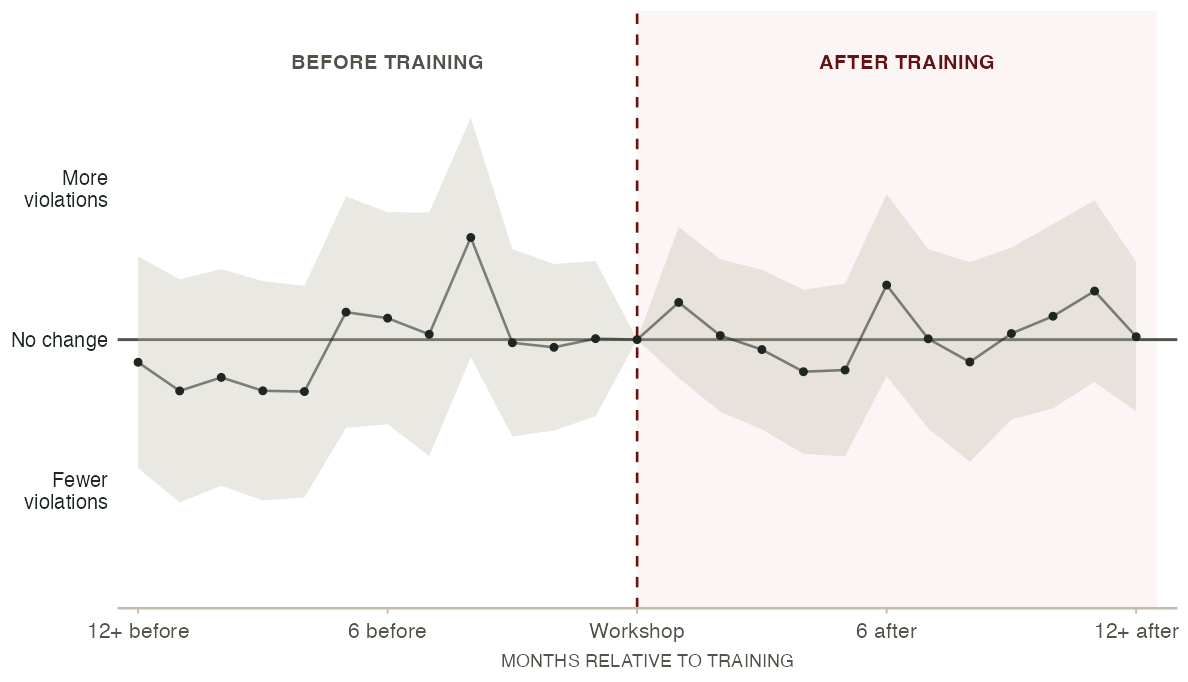
\includegraphics[width=\linewidth]{../../data-viz/figures/fig2-event-study.png}
\par\vspace{3pt}
{\color{faint}\fontsize{7.1pt}{9.5pt}\selectfont \textit{Note:} Each dot shows whether facilities had more or fewer violations in a given month relative to the workshop month. The estimates account for each facility's usual number of violations, the local weather, and any common trends shared across facilities; the shaded band shows the range of estimates within the 95\% confidence interval. If the workshops had reduced violations, the line would drop below zero after the workshop.\par}
\end{minipage}
\end{center}

\vspace{6pt}

While compliance assistance programs presume that facilities violate because they do not fully understand the rules, Ferraro and Shimshack find no support for that view: the workshops supplied the technical guidance facilities were supposedly lacking, and neither violations nor discharges changed. At least \textbf{in this context, a lack of facility understanding does not appear to be what was holding compliance back.}

\begin{moreinfo}
Contact Jay Shimshack (jay.shimshack@virginia.edu) with questions about this research.\par

Ferraro, Paul J., and Jay P. Shimshack. 2026. ``The Effect of Compliance Assistance on Pollution Discharges and Violations of Environmental Regulations.'' \textit{Journal of Policy Analysis and Management} 45 (3): e70056. \href{https://doi.org/10.1002/pam.70056}{\color{cite}\underline{doi.org/10.1002/pam.70056}}.\par

\textbf{Paul J. Ferraro} is the Bloomberg Distinguished Professor of Human Behavior and Public Policy at Johns Hopkins University, Carey Business School and Department of Environmental Health and Engineering, and Bloomberg School of Public Health \& Whiting School of Engineering.\par
\textbf{Jay P. Shimshack} is a Professor of Public Policy and Economics at Frank Batten School of Leadership and Public Policy at the University of Virginia.\par

The \href{https://www.environmental-inequality-lab.org/}{\color{cite}\underline{Environmental Inequality Lab}} is a nonpartisan research group that applies a rigorous, data-driven approach to understand how our environment shapes economic opportunity and well-being.\par
\end{moreinfo}




\end{document}
